\begin{figure}[!t]
\centering
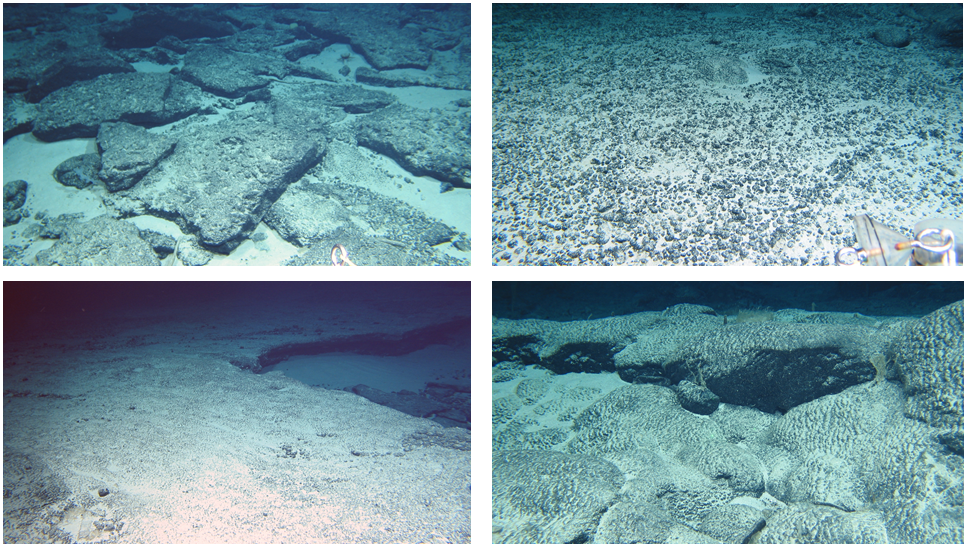
\includegraphics[width=5.5in]{./images/mehul1.png}
\caption{Different seafloor terrain at Takuyo Daigo seamount\cite{Thornton2013l}. . Clockwise, from top left: Broken slabs in sand, nodules, pillowy crusts and continuous flat crusts}
\label{f:mehul1}
\end{figure}
The complexity of seafloor topology (see Fig.~\ref{f:mehul1}) prohibits vehicles from simply landing at random locations and requires the identification and intelligent choice of landing sites. At the same time, the spatial scales relevant to AUV landing are too small to be observed by ship-board acoustic multibeam. Therefore, in order for an AUV to identify landing sites during its survey, it should be equipped with a mapping system capable of generating bathymetry with sufficiently high resolution, e.g. using light sectioning \cite{Inglis2012,Nishida2016,Bodenmann2016}. Even though landing site detection for aerial vehicles has been studied in \cite{Desaraju2014, Sharp2001}, the conditions essential for safe landing in underwater environments has not been sufficiently investigated. Simulations for control, navigation and dynamics of AUVs with landing capabilities have been reported in \cite{Wang2007, Du2012}. However, these previous works do not develop the sensing and data processing methods needed to automatically identify areas where a vehicle can land safely. Regarding methods to analyse seafloor terrains, Fourier analysis based segmentation and 3D alignment was described in \cite{Douillard2012,Douillard2013}. Other methods for surface classification using wavelets \cite{Bhandari2007} have also been described, but have not been applied to landing site identification. Early works by our group demonstrated a landing algorithm using Fourier analysis to separate flat ground surface from objects on the seafloor \cite{Sangekar2010c}. The algorithm rejected all protruding objects as non-landable areas, and only considered flat regions for landing. This work builds on our previous studies, identifying the geometric conditions where it is possible to land on protruding objects and to land on slopes, considering the vehicle's righting moment. 


The remainder of this paper is organized as follows; Section II describes the hardware requirements for landing, including the conceptual design of an underwater vehicle capable of landing and its high resolution mapping system for generating bathymetry with mm-resolution. In  Section III, the different steps of the algorithm to identify landing sites are described and demonstrated by simulating its performance on seafloor data obtained using an equivalent high resolution mapping system.  Section IV applies the algorithm to more than 1000\,m$^2$ of seafloor bathymetry obtained using an AUV during an underwater survey. Section V presents the conclusions of this work. 
% However, the large localization uncertainty \cite{Masmitja2016} associated with deep sea operations means that landing sites determined prior to deployment cannot be reached with sufficient navigational accuracy.
